%! Author = chtompki
%! Date = 1/14/26
\documentclass[10pt]{amsart}
% Default margins are too wide all the way around. I reset them here
\setlength{\hoffset}{-.75in}
\setlength{\textwidth}{6.5in}
\setlength{\voffset}{-.5in}
\setlength{\textheight}{9.0in}
\usepackage{amsmath}
\usepackage{amssymb}
\usepackage{amsthm}
\usepackage{lmodern}
\usepackage{microtype}
\usepackage{enumitem}
\usepackage{setspace}
\usepackage{graphicx}
\usepackage{hyperref}
\usepackage{tikz}
\usepackage{listings}
\usepackage{pgfplots}
\pgfplotsset{compat=1.18}
\usepgfplotslibrary{groupplots}


\newenvironment{solution}
{\begin{proof}[Solution]}
{\end{proof}}

\NewDocumentCommand{\vitem}{v}{%
    \item[\texttt{#1}]%
}

\newcommand{\slopeelement}[3]{%
    \pgfmathsetmacro{\slopeDX}{0.14/sqrt(1+(#3)^2)}%
    \pgfmathsetmacro{\slopeDY}{(#3)*\slopeDX}%
    \pgfmathsetmacro{\slopeXA}{(#1)-\slopeDX}%
    \pgfmathsetmacro{\slopeYA}{(#2)-\slopeDY}%
    \pgfmathsetmacro{\slopeXB}{(#1)+\slopeDX}%
    \pgfmathsetmacro{\slopeYB}{(#2)+\slopeDY}%
    \edef\slopecommand{%
        \noexpand\draw[gray,thin]
        (axis cs:\slopeXA,\slopeYA)
        --
        (axis cs:\slopeXB,\slopeYB);%
    }%
    \slopecommand
}

\title{Dynamical Systems\\Problem Set 2}
\author{Rob Tompkins}
\date{\today}

\begin{document}
    \maketitle
    \date{\today}
    \begin{onehalfspace}
        We begin by noting that all of the files referenced in this document are available at: \\
        \underline{https://github.com/chtompki/MathFall2026/tree/main/DynamicalSystems/ProblemSet2}

        The next exercises (3.4.5, 3.5.7, and 3.4.9) are designed to test your ability to distinguish among the various
        types of bifurcations --- its easy to confuse them!
        In each case, fine the values of $r$ at which bifurcations occur, and classify those as: saddle-node,
        transcritical, supercritical pitchfork, or subcritical pitchfork.
        Finally sketch the bifurcation diagram of fixed points $x^*$ vs $r$.

        \noindent\textbf{3.4.5} $\dot{x} = r - 3x^2$

        \begin{solution}
Fixed points satisfy $x^*=\pm\sqrt{r/3}$ for $r\ge0$. Since $f_x=-6x$, the positive branch is stable and the negative branch unstable. The two coalesce at $r=0$, so this is a saddle-node bifurcation.

\medskip
\begin{center}
\begin{tikzpicture}
\begin{axis}[width=9cm,height=6cm,axis lines=middle,xlabel={$r$},ylabel={$x^*$},
xmin=-0.5,xmax=3.2,ymin=-1.2,ymax=1.2,samples=160]
\addplot[thick,domain=0:3] {sqrt(x/3)};
\addplot[thick,dashed,domain=0:3] {-sqrt(x/3)};
\addplot[only marks,mark=*] coordinates {(0,0)};
\end{axis}
\end{tikzpicture}

\small Solid is stable; dashed is unstable.
\end{center}

\end{solution}

        \noindent\textbf{3.4.7} $\dot{x} = 5 - re^{-x^2}$

        \begin{solution}
Fixed points require $e^{-x^2}=5/r$. Thus none exist for $r<5$, one ($x=0$) exists at $r=5$, and for $r>5$,
\[x^*=\pm\sqrt{\ln(r/5)}.\]
Since $f_x=2rxe^{-x^2}=10x$ at equilibrium, the negative branch is stable and the positive branch unstable. Hence $r=5$ is a saddle-node bifurcation.

\medskip
\begin{center}
\begin{tikzpicture}
\begin{axis}[width=9cm,height=6cm,axis lines=middle,xlabel={$r$},ylabel={$x^*$},
xmin=3.5,xmax=12,ymin=-1.1,ymax=1.1,samples=180]
\addplot[thick,dashed,domain=5.001:12] {sqrt(ln(x/5))};
\addplot[thick,domain=5.001:12] {-sqrt(ln(x/5))};
\addplot[only marks,mark=*] coordinates {(5,0)};
\node[anchor=south west] at (axis cs:5,0) {$r=5$};
\end{axis}
\end{tikzpicture}

\small The lower branch is stable and the upper branch is unstable.
\end{center}

\end{solution}

        \noindent\textbf{3.4.9} $\dot{x} = x = \tanh{(rx)}$

        \begin{solution}
For $f=x+\tanh(rx)$, $x=0$ is always fixed and $f_x(0)=1+r$, so the critical value is $r=-1$. Using
\[\tanh(rx)=rx-\frac{r^3x^3}{3}+O(x^5),\]
we get near $r=-1$ the normal form $\dot x\approx\mu x+x^3/3$, where $\mu=r+1$. Therefore the bifurcation at $r=-1$ is a subcritical pitchfork: the origin is stable for $r<-1$ and unstable for $r>-1$, with two unstable nonzero branches on the $r<-1$ side.

\medskip
The nonzero fixed points may be plotted implicitly from
\[
r=-\frac{\operatorname{arctanh}(x^*)}{x^*}.
\]
\begin{center}
\begin{tikzpicture}
\begin{axis}[width=9cm,height=6cm,axis lines=middle,xlabel={$r$},ylabel={$x^*$},
xmin=-3.2,xmax=0.5,ymin=-1.05,ymax=1.05,samples=180]
\addplot[thick] coordinates {(-3.2,0) (-1,0)};
\addplot[thick,dashed] coordinates {(-1,0) (0.5,0)};
\addplot[thick,dashed,domain=0.03:0.95,variable=\u]
({-0.5*ln((1+\u)/(1-\u))/\u},{\u});
\addplot[thick,dashed,domain=-0.95:-0.03,variable=\u]
({-0.5*ln((1+\u)/(1-\u))/\u},{\u});
\addplot[only marks,mark=*] coordinates {(-1,0)};
\end{axis}
\end{tikzpicture}

\small Subcritical pitchfork at $r=-1$: solid is stable and dashed is unstable.
\end{center}

\end{solution}

        \noindent\textbf{3.4.11} (An interesting bifurcation diagram) Consider $\dot{x} = rx - \sin{(x)}$
        \begin{itemize}
            \item[a)] For the case $r = 0$, find and classify all the fixed points, and sketch the vector field.
            \item[b)] Show that when $r > 1$, there is only one fixed point.
            What kind of fixed point is it?
            \item[c)] As $r$ decreases from $\infty$ to $0$, classify \emph{all} the bifurcations that occur.
            \item[d)] For $0 < r \ll 1$, find an approximate formula for all values of $r$ at which bifurcations occur.
            \item[e)] Now classify all the bifurcations that occur as $r$ decreases from $0$ to $-\infty$.
            \item[f)] Plot the bifurcation diagram for $-\infty < r < \infty$, and indicate the stability of the various
            fixed points.
        \end{itemize}

        \begin{solution}
Let $f=rx-\sin x$.
\begin{enumerate}[label=(\alph*)]
\item At $r=0$, $x^*=n\pi$. Since $f_x=-\cos x$, $2k\pi$ is stable and $(2k+1)\pi$ unstable.
\item If $r>1$, $|\sin x/x|\le1<r$ for $x\ne0$, so only $x=0$ remains; it is unstable because $f_x(0)=r-1>0$.
\item Saddle-nodes satisfy $f=f_x=0$, hence $rx=\sin x$, $r=\cos x$, and therefore $\tan x=x$. At the origin, $f=(r-1)x+x^3/6+\cdots$, so $r=1$ is a subcritical pitchfork.
\item For small positive $r$, roots of $\tan x=x$ lie near $a_n=(2n+\tfrac12)\pi$. Writing $x_n=a_n-\varepsilon_n$ gives $\varepsilon_n\sim1/a_n$, hence
\[r_n\approx\frac{1}{(2n+\tfrac12)\pi}.\]
\item For $r<0$, saddle-nodes again satisfy $\tan x=x$, now with $r=\cos x<0$; these values accumulate at $0$ from below.
\item The diagram is symmetric in $x$. The branch $x=0$ is stable for $r<1$ and unstable for $r>1$; the other branches terminate in the saddle-nodes described above. Stability follows from the sign of $r-\cos x$.
\end{enumerate}

\medskip
The complete equilibrium curve is
\[
r=\frac{\sin x^*}{x^*},\qquad r(0)=1.
\]
\begin{center}
\begin{tikzpicture}
\begin{axis}[width=10cm,height=7cm,axis lines=middle,xlabel={$r$},ylabel={$x^*$},
xmin=-0.3,xmax=1.1,ymin=-16,ymax=16,samples=700]
\addplot[thick,domain=-15.7:-0.08,variable=\u] ({sin(deg(\u))/\u},{\u});
\addplot[thick,domain=0.08:15.7,variable=\u] ({sin(deg(\u))/\u},{\u});
\addplot[thick] coordinates {(-0.3,0) (1,0)};
\addplot[thick,dashed] coordinates {(1,0) (1.1,0)};
\addplot[only marks,mark=*] coordinates {(1,0)};
\end{axis}
\end{tikzpicture}

\small Stability along each segment is determined by the sign of $r-\cos x^*$.
\end{center}

\end{solution}

        \noindent\textbf{3.4.14} (Subcritical pitchfork) Consider the system $\dot{x} = rx + x^3 -x^5$, which
        exhibits a subcritical pitchfork bifurcation.
        \begin{itemize}
            \item[a)] Find algebraic expressions for the all the fixed points at $r$ varies.
            \item[b)] Sketch the vector fields as $r$ varies.
            Be sure to indicate all the fixed points and their stability.
            \item[c)] Calculate $r_s$, the parameter value at which the nonzero fixed points are born in a saddle-node
            bifurcation.
        \end{itemize}

        \begin{solution}
Write $\dot x=x(r+x^2-x^4)$.
\begin{enumerate}[label=(\alph*)]
\item Besides $x=0$, put $u=x^2$. Then $u^2-u-r=0$, so
\[x^*=\pm\sqrt{\frac{1\pm\sqrt{1+4r}}{2}}.\]
The outer pair exists for $r\ge-1/4$ and the inner pair for $-1/4\le r\le0$.
\item At $x=0$, $f_x=r$. At a nonzero fixed point, $f_x=2x^2(1-2x^2)$, so the inner pair is unstable and outer pair stable. Thus two saddle-nodes occur at $r=-1/4$, and the inner pair joins the origin in the subcritical pitchfork at $r=0$.
\item The saddle-node value is
\[r_s=-\frac14,\]
with $x=\pm1/\sqrt2$.
\end{enumerate}

\medskip
\begin{center}
\begin{tikzpicture}
\begin{axis}[width=10cm,height=7cm,axis lines=middle,xlabel={$r$},ylabel={$x^*$},
xmin=-0.32,xmax=0.55,ymin=-1.45,ymax=1.45,samples=180]
\addplot[thick] coordinates {(-0.32,0) (0,0)};
\addplot[thick,dashed] coordinates {(0,0) (0.55,0)};
\addplot[thick,domain=-0.25:0.55] {sqrt((1+sqrt(1+4*x))/2)};
\addplot[thick,domain=-0.25:0.55] {-sqrt((1+sqrt(1+4*x))/2)};
\addplot[thick,dashed,domain=-0.25:0] {sqrt((1-sqrt(1+4*x))/2)};
\addplot[thick,dashed,domain=-0.25:0] {-sqrt((1-sqrt(1+4*x))/2)};
\addplot[only marks,mark=*] coordinates {(-0.25,0.707106) (-0.25,-0.707106) (0,0)};
\end{axis}
\end{tikzpicture}

\small Solid branches are stable; dashed branches are unstable.
\end{center}

\end{solution}

        \noindent\textbf{3.4.16} (Potentials) In parts (a)-(c) let $V(x)$ be the potential, in the sense that
        $\dot{x} = -dV/dx$.
        Sketch the potential as a function of $r$.
        Show all qualitatively different cases including bifurcation values of $r$.
        \begin{itemize}
            \item[a)] (Saddle-node) $\dot{x} = r - x^2$
            \item[b)] (Transcritical) $\dot{x} = rx - x^2$
            \item[c)] (Subcritical pitchfork) $\dot{x} = rx + x^3 - x^5$.
        \end{itemize}

        \begin{solution}
Since $\dot x=-V'(x)$:
\begin{enumerate}[label=(\alph*)]
\item $V=x^3/3-rx+C$. For $r>0$ it has a maximum at $-\sqrt r$ and minimum at $\sqrt r$; these merge at $r=0$.
\item $V=-rx^2/2+x^3/3+C$. The stationary points $0$ and $r$ exchange maximum/minimum character at $r=0$.
\item $V=-rx^2/2-x^4/4+x^6/6+C$. The qualitative changes occur at $r=-1/4$ and $r=0$: for $-1/4<r<0$ there are three minima separated by two maxima; for $r>0$ the origin is a maximum and the two outer equilibria are minima.
\end{enumerate}

\medskip
Representative potential curves (additive constants are irrelevant) are:
\begin{center}
\begin{tikzpicture}
\begin{groupplot}[group style={group size=3 by 1,horizontal sep=0.8cm},
width=5cm,height=4.3cm,axis lines=middle,samples=150,xtick=\empty,ytick=\empty]
\nextgroupplot[title={saddle-node},xmin=-2,xmax=2,ymin=-2,ymax=2]
\addplot[thick,domain=-2:2] {x^3/3-x};
\nextgroupplot[title={transcritical},xmin=-2,xmax=2,ymin=-1.2,ymax=2]
\addplot[thick,domain=-2:2] {-x^2/2+x^3/3};
\nextgroupplot[title={subcritical pitchfork},xmin=-1.7,xmax=1.7,ymin=-0.5,ymax=1.2]
\addplot[thick,domain=-1.7:1.7] {0.08*x^2-x^4/4+x^6/6};
\end{groupplot}
\end{tikzpicture}
\end{center}

\end{solution}

        \noindent\textbf{3.5.4} (Bead on a horizontal wire) A bead of mass $m$  is constrained to slide along
        a straight horizontal wire.
        A spring of relaxed length $L_0$ and spring constant $k$ is attached to the mass and to a support point
        distance $h$ from the wire given in Figure \ref{figure1} below.

        \begin{figure}[htbp]
            \centering
            \IfFileExists{figure1.jpeg}{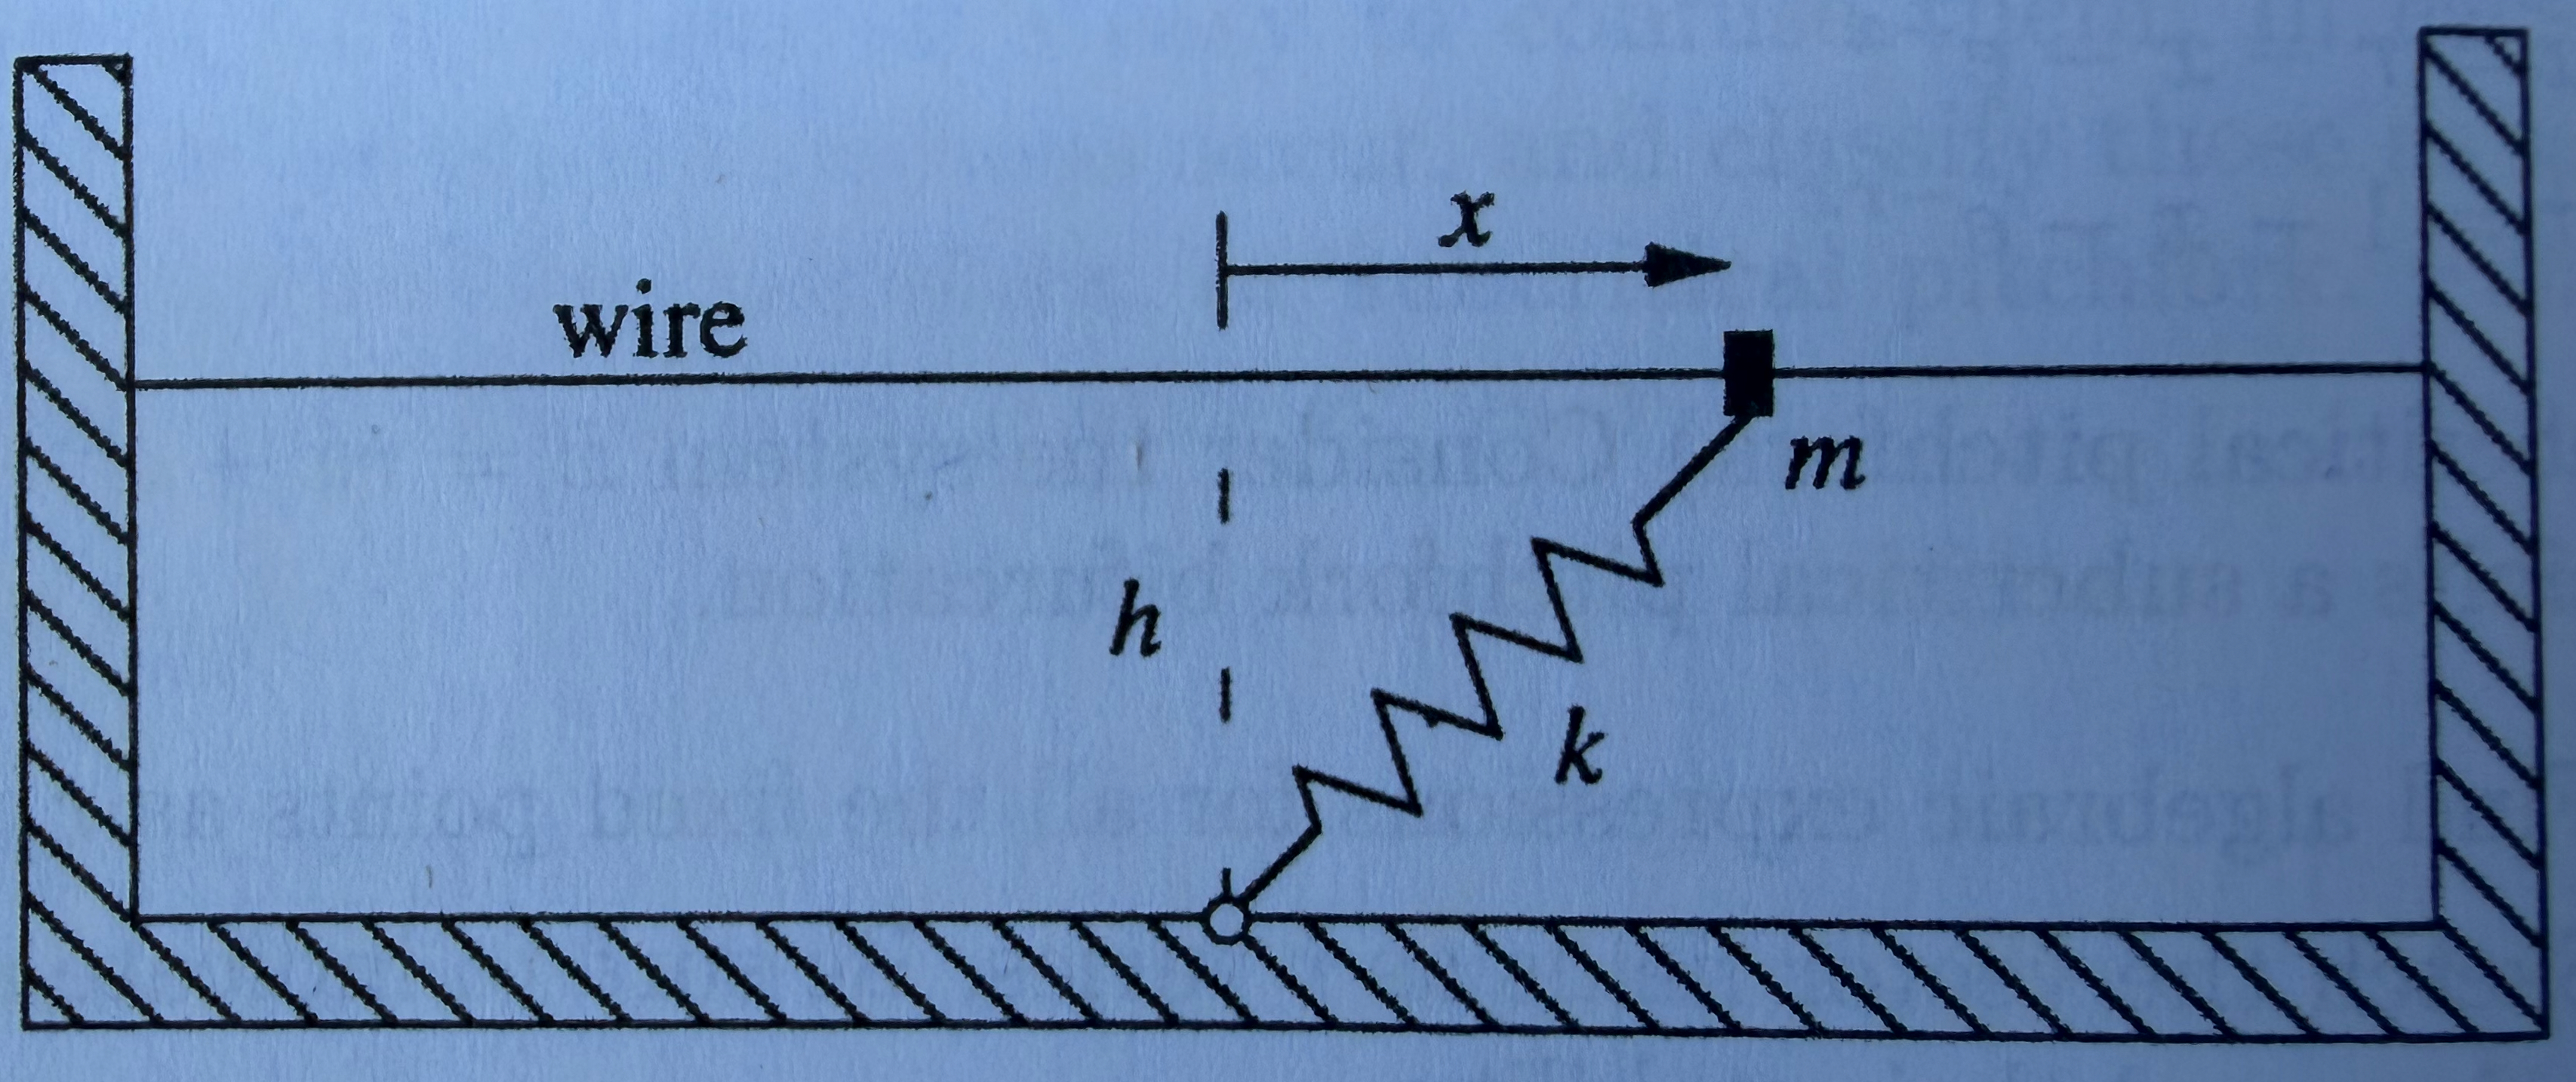
\includegraphics[width=\textwidth]{figure1.jpeg}}{\fbox{\parbox{0.9\textwidth}{Figure 1 from the original assignment goes here.}}}
            \caption{}
            \label{figure1}
        \end{figure}

        \noindent Finally suppose that the motion of the bead is opposed by a viscous damping force $b\dot{x}$.
        \begin{itemize}
            \item[a)] Write Newton's law for the motion of the fixed bead.
            \item[b)] Find all possible equilibria, i.e. fixed points, as functions of $k$, $h$, $m$, $b$, and $L_0$.
            \item[c)] Suppose $m = 0$.
            Classify the stability of all the fixed points, and draw a bifurcation diagram.
            \item[d)] If $m\neq 0$, how small must $m$ be, to be considered negligible?
            In what sense is it negligible?
        \end{itemize}

        \begin{solution}
Let $\ell=\sqrt{x^2+h^2}$.
\begin{enumerate}[label=(\alph*)]
\item Newton's law is
\[m\ddot x+b\dot x+kx\left(1-\frac{L_0}{\sqrt{x^2+h^2}}\right)=0.\]
\item Equilibria satisfy $x(1-L_0/\ell)=0$, so $x=0$ always and, if $L_0\ge h$,
\[x=\pm\sqrt{L_0^2-h^2}.\]
\item If $m=0$, $f'(0)=-(k/b)(1-L_0/h)$. Thus the origin is stable for $L_0<h$ and unstable for $L_0>h$, while the two nonzero equilibria are stable. Hence $L_0=h$ is a supercritical pitchfork.
\item Inertia is negligible when its relaxation time $m/b$ is much shorter than the overdamped time $b/k$, i.e.
\[\frac{mk}{b^2}\ll1.\]
Then inertia matters only during a short initial transient.
\end{enumerate}
\end{solution}

        \noindent\textbf{3.6.2} (Imperfect transcritical bifurcation) Consider the system $\dot{x} = h + rx - x^2$.
        When $h = 0$, this system undergoes a transcritical bifurcation at $r = 0$.
        Our goal is to see how the bifurcation diagram of $x^*$ vs. $r$ is affected by the imperfection parameter $h$.
        \begin{itemize}
            \item[a)] Plot the bifurcation diagram for $\dot{x} = h + rx - x^2$, for $h < 0$, $h = 0$, and $h > 0$.
            \item[b)] Sketch the regions in the $(r,h)$ plane that correspond to qualitatively different vector fields,
            and identify the bifurcation that occur on the boundaries of those regions.
            \item[c)] Plot the potential $V(x)$ corresponding to all the different regions in the $(r,h)$ plane.
        \end{itemize}

        \begin{solution}
The fixed points are
\[x^*_{\pm}=\frac{r\pm\sqrt{r^2+4h}}2.\]
\begin{enumerate}[label=(\alph*)]
\item For $h>0$ there are always two fixed points, with $x_+$ stable and $x_-$ unstable. For $h=0$, $x=0$ and $x=r$ exchange stability at the transcritical bifurcation $r=0$. For $h<0$, saddle-nodes occur at $r=\pm2\sqrt{-h}$; there are no fixed points between them.
\item The bifurcation set in parameter space is
\[h=-\frac{r^2}{4}.\]
Above it are two fixed points, on it one double fixed point, and below it none. Away from the origin the boundary consists of saddle-node bifurcations.
\item The potential is
\[V(x)=-hx-\frac r2x^2+\frac13x^3+C.\]
Two stationary points occur when $r^2+4h>0$, one degenerate stationary point on the parabola, and none below it.
\end{enumerate}

\medskip
\begin{center}
\begin{tikzpicture}
\begin{groupplot}[group style={group size=3 by 1,horizontal sep=0.8cm},
width=5cm,height=4.7cm,axis lines=middle,xlabel={$r$},ylabel={$x^*$},
xmin=-3,xmax=3,ymin=-3,ymax=3,samples=160]
\nextgroupplot[title={$h=-1/2$}]
\addplot[thick,domain=-3:-1.415] {(x+sqrt(x^2-2))/2};
\addplot[thick,dashed,domain=-3:-1.415] {(x-sqrt(x^2-2))/2};
\addplot[thick,domain=1.415:3] {(x+sqrt(x^2-2))/2};
\addplot[thick,dashed,domain=1.415:3] {(x-sqrt(x^2-2))/2};
\nextgroupplot[title={$h=0$}]
\addplot[thick] coordinates {(-3,0) (0,0)};
\addplot[thick,dashed] coordinates {(0,0) (3,0)};
\addplot[thick,dashed] coordinates {(-3,-3) (0,0)};
\addplot[thick] coordinates {(0,0) (3,3)};
\nextgroupplot[title={$h=1/2$}]
\addplot[thick,domain=-3:3] {(x+sqrt(x^2+2))/2};
\addplot[thick,dashed,domain=-3:3] {(x-sqrt(x^2+2))/2};
\end{groupplot}
\end{tikzpicture}

\small Solid branches are stable; dashed branches are unstable.
\end{center}

\begin{center}
\begin{tikzpicture}
\begin{axis}[width=8cm,height=5cm,axis lines=middle,xlabel={$r$},ylabel={$h$},
xmin=-3,xmax=3,ymin=-2.5,ymax=1,samples=150]
\addplot[thick,domain=-3:3] {-x^2/4};
\node at (axis cs:0,0.55) {two fixed points};
\node at (axis cs:0,-1.4) {no fixed points};
\end{axis}
\end{tikzpicture}
\end{center}

\end{solution}

        \noindent\textbf{3.7.5} (A biochemical switch) Zebra stripes and butterfly wing patterns are two of the most
        spectacular examples of biological pattern formation.
        Explaining the development of these patterns is on of the outstanding problems of Biology; see Murray (2003)
        for an excellent review.

        As one ingredient in a model of pattern formation, Lewis et al. (1977) considered a simple example of a
        biochemical switch, in which a gene $G$ is activated by a biochemical signal substance $S$.
        For example, the gene may normally be inactive but can be ``switched on'' to produce a pigment or other gene
        product when concentration of $S$ exceeds a certain threshold.
        Let $g(t)$ denote the concentration of the gene product, and assume that the concentration $s_0$ of $S$ is
        fixed.
        The model is
        \[
            \dot{g} = k_1 s_0 - k_2 g + \frac{k_3 g^2}{k_4^2 + g^2},
        \]
        where $k$'s are positive constants.
        The production of $g$ is stimulated by $s_0$ at rate $k_1$, and by an \emph{autocatalytic} (positive feedback)
        process, modeled by the non-linear term.
        There is also a linear degradation of $g$ at a rate $k_2$.
        \begin{itemize}
            \item[a)] Show that the system can be put in the dimensionless form
            \[
                \frac{dx}{d\tau} = s - rx + \frac{x^2}{1+x^2},
            \]
            where $r > 0$ and $s\ge 0$ are dimensionless groups.
            \item[b)] Show that if $s = 0$, there are two positibe fixed points $x^*$ if $r < r_c$, where $r_c$ is to
            be determined.
            \item[c)] Assume that initially there is no gene product, i.e. $g(0) = 0$, ad suppose $s$ is slowly
            increased from $0$ (the activating signal is turned on); what happens to $g(t)$?
            What happens if $s$ then goes back to zero?
            Does the gene turn off again?
            \item[d)] Find parametric equations for the bifurcation curves in $(r, s)$ space, and classify
            the bifurcations that occur.
            \item[e)] Compute a quantitatively accurate plot of the stability diagram in $(r, s)$ space.
        \end{itemize}
        For further discussion of this model, see Lewis et al. (1977); Edelstein-Kishet (1988); Section 7.5; or
        Murray (2002), Chapter 6.

        \begin{solution}
\begin{enumerate}[label=(\alph*)]
\item Let $x=g/k_4$ and $\tau=(k_3/k_4)t$. Then
\[\frac{dx}{d\tau}=s-rx+\frac{x^2}{1+x^2},\qquad s=\frac{k_1s_0}{k_3},\quad r=\frac{k_2k_4}{k_3}.\]
\item For $s=0$, positive fixed points satisfy $r=x/(1+x^2)$. This has maximum $1/2$ at $x=1$, so $r_c=1/2$ and two positive fixed points exist for $0<r<1/2$.
\item Slowly increasing $s$ follows the low stable branch until a saddle-node causes a jump to the high branch. On decreasing $s$ again, the system can remain on the high branch: the switch exhibits hysteresis.
\item From $f=f_x=0$,
\[r(x)=\frac{2x}{(1+x^2)^2},\qquad s(x)=\frac{x^2(1-x^2)}{(1+x^2)^2}.\]
These parameterize the saddle-node curves.
\item The cusp satisfies $dr/dx=0$, giving $x=1/\sqrt3$ and
\[(r,s)=\left(\frac{3\sqrt3}{8},\frac18\right).\]
Inside the cusp region there are three fixed points (two stable, one unstable); outside there is one.
\end{enumerate}

\medskip
The saddle-node boundary is given parametrically by the formulas above:
\begin{center}
\begin{tikzpicture}
\begin{axis}[width=8.5cm,height=6cm,axis lines=middle,xlabel={$r$},ylabel={$s$},
xmin=0,xmax=0.72,ymin=0,ymax=0.145,samples=220]
\addplot[thick,domain=0.001:1,variable=\u]
({2*\u/(1+\u^2)^2},{\u^2*(1-\u^2)/(1+\u^2)^2});
\addplot[only marks,mark=*] coordinates {(0.649519,0.125)};
\node[anchor=south west] at (axis cs:0.649519,0.125)
{$\left(\frac{3\sqrt3}{8},\frac18\right)$};
\node at (axis cs:0.50,0.075) {\scriptsize three fixed points};
\end{axis}
\end{tikzpicture}
\end{center}

\end{solution}

        \noindent\textbf{5.1.10} (Attracting and Liapunov stable) here are the official definitions of various
        types of stability.
        Consider a fixed point $\mathbf{x^*}$ of a system $\mathbf{\dot{x} = f(x)}$.

        \noindent We say that $\mathbf{x^*}$ is \textbf{\emph{attracting}} if there is a $\delta >0$ such that
        $\lim\limits_{t\rightarrow\infty} x(t) = \mathbf{x^*}$ whenever $\|\mathbf{x}(0) - \mathbf{x^*}\| < \delta$
        within a distance of $\delta$ to $\mathbf{x^*}$ is guaranteed to converge to $\mathbf{x^*}$ \emph{eventually}.
        As shown schematically in Figure \ref{figure2}, trajectories that start nearby are allowed to stray from
        $\mathbf{x^*}$ in the short run, but the must approach $\mathbf{x^*}$ in the long run.

        \noindent In contrast, Liapunov stability requires that nearby trajectories remain close for \emph{all} time.
        We sayt that $\mathbf{x^*}$ is \textbf{\emph{Liapunov stable}} if for each $\varepsilon > 0$ there is a
        $\delta > 0$ such that $\|\mathbf{x}(t) - \mathbf{x^*}\| < \varepsilon$ whenever $t \ge 0$ and
        $\|\mathbf{x}(0) - \mathbf{x^*}\| < \delta$.
        Thus, trajectories that start within $\delta$ of $\mathbf{x^*}$ remain within $\varepsilon$ of $\mathbf{x^*}$
        for all positive time.
        Figure \ref{figure2} gives a good example of this
        \begin{figure}[htbp]
            \centering
            \IfFileExists{figure2.png}{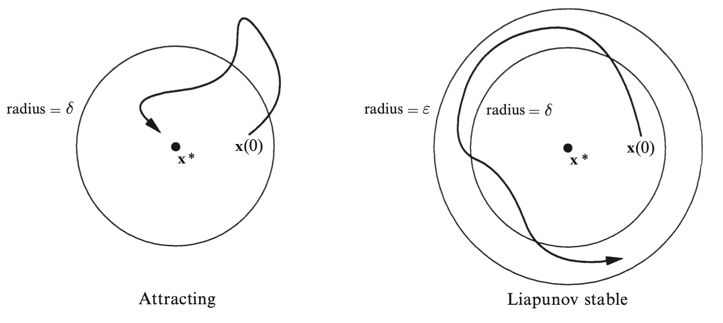
\includegraphics[width=\textwidth]{figure2.png}}{\fbox{\parbox{0.9\textwidth}{Figure 2 from the original assignment goes here.}}}
            \caption{}
            \label{figure2}
        \end{figure}
        Finally $\mathbf{x^*}$ is \textbf{\emph{asymptotically stable}} if it is both attracting and Liapunov stable.

        \noindent For each of the following systems, decide whether the origin is attracting, Liapunov stable,
        asymptotically stable, or none of the above.
        \begin{itemize}
            \item[a)] $\dot{x} = y$, $\dot{y} = -4x$
            \item[b)] $\dot{x} = 2y$, $\dot{y} = x$
            \item[c)] $\dot{x} = 0$, $\dot{y} = x$
            \item[d)] $\dot{x} = 0$, $\dot{y} = -y$
            \item[e)] $\dot{x} = -x$, $\dot{y} = -5y$
            \item[f)] $\dot{x} = x$, $\dot{y} = y$
        \end{itemize}

        \begin{solution}
\begin{enumerate}[label=(\alph*)]
\item Eigenvalues $\pm2i$: closed ellipses. The origin is Liapunov stable but not attracting.
\item Eigenvalues $\pm\sqrt2$: saddle. The origin is neither attracting nor Liapunov stable.
\item $x=x_0$, $y=y_0+x_0t$: the origin is neither attracting nor Liapunov stable.
\item $x=x_0$, $y=y_0e^{-t}$: Liapunov stable but not attracting.
\item $x=x_0e^{-t}$, $y=y_0e^{-5t}$: asymptotically stable, hence attracting and Liapunov stable.
\item $x=x_0e^t$, $y=y_0e^t$: neither attracting nor Liapunov stable.
\end{enumerate}
\end{solution}

        \noindent\textbf{5.2.1} Consider the system $\dot{x} = 4x - y$, $\dot{y} = 2x + y$.
        \begin{itemize}
            \item[a)] Write the system as $\mathbf{\dot{x}} = A \mathbf{x}$.
            Show that the characteristic equation is $\lambda^2 - 5\lambda + 6 = 0$,
            and find the eigenvalues and eigenvectors of $A$.
            \item[b)] Find the general solution of the system.
            \item[c)] Classify the fixed point at the origin.
            \item[d)] Solve the system subject ot the initial condition $(x_0, y_0) = (3, 4)$.
        \end{itemize}

        \begin{solution}
\begin{enumerate}[label=(\alph*)]
\item
\[A=\begin{pmatrix}4&-1\\2&1\end{pmatrix},\qquad \det(A-\lambda I)=\lambda^2-5\lambda+6.\]
Thus $\lambda=2,3$, with eigenvectors $(1,2)^T$ and $(1,1)^T$, respectively.
\item
\[\mathbf{x}(t)=c_1e^{2t}\begin{pmatrix}1\\2\end{pmatrix}+c_2e^{3t}\begin{pmatrix}1\\1\end{pmatrix}.\]
\item Both eigenvalues are positive, so the origin is an unstable node.
\item From $(3,4)$, $c_1=1$, $c_2=2$. Hence
\[x(t)=e^{2t}+2e^{3t},\qquad y(t)=2e^{2t}+2e^{3t}.\]
\end{enumerate}
\end{solution}

        \noindent\textbf{5.2.6} Plot the phase portrait and classify the fixed point of the following
        linear systems.
        If the eigenvectors are real, indicate them in your sketch.
        \begin{eqnarray*}
            \dot{x} & = & -3x + 2y \\
            \dot{y} & = & x - 2y
        \end{eqnarray*}

        \begin{solution}
Here
\[A=\begin{pmatrix}-3&2\\1&-2\end{pmatrix},\]
and
\[\det(A-\lambda I)=\lambda^2+5\lambda+4=(\lambda+1)(\lambda+4).\]
Thus $\lambda_1=-1$ with eigenvector $(1,1)^T$, and $\lambda_2=-4$ with eigenvector $(-2,1)^T$. Both eigenvalues are real, distinct, and negative, so the origin is a stable node. The phase portrait has invariant straight lines along $y=x$ and $y=-x/2$, and all trajectories approach the origin as $t\to\infty$, asymptotically tangent to the slower eigendirection $y=x$.

\medskip
\begin{center}
\begin{tikzpicture}
\begin{axis}[width=8cm,height=8cm,axis equal image,axis lines=middle,
xlabel={$x$},ylabel={$y$},xmin=-2,xmax=2,ymin=-2,ymax=2]
\addplot[thick,domain=-2:2] {x};
\addplot[thick,dashed,domain=-2:2] {-x/2};
\addplot[only marks,mark=*] coordinates {(0,0)};
\draw[-stealth] (axis cs:1.6,1.6) -- (axis cs:0.9,0.9);
\draw[-stealth] (axis cs:-1.6,-1.6) -- (axis cs:-0.9,-0.9);
\draw[-stealth] (axis cs:1.6,-0.8) -- (axis cs:0.8,-0.4);
\draw[-stealth] (axis cs:-1.6,0.8) -- (axis cs:-0.8,0.4);
\draw[-stealth] (axis cs:1.5,0.4) -- (axis cs:0.7,0.25);
\draw[-stealth] (axis cs:-1.5,-0.4) -- (axis cs:-0.7,-0.25);
\draw[-stealth] (axis cs:0.4,1.5) -- (axis cs:0.2,0.65);
\draw[-stealth] (axis cs:-0.4,-1.5) -- (axis cs:-0.2,-0.65);
\end{axis}
\end{tikzpicture}

\small The solid line is the slow eigendirection $y=x$ and the dashed line is
$y=-x/2$. All trajectories approach the origin.
\end{center}

\end{solution}

    \end{onehalfspace}
\end{document}